\documentclass[../main.tex]{subfiles}

\begin{document}

\chapquote{Chess is the struggle against the error.}{Johannes Zukertort}
\chapter{Evaluation}
\label{chap:evaluation}

\begin{table}
    \makebox[\textwidth][c]{
        \begin{tabular}{lrrr}
            \toprule
            metric & train & val & test \\
            \midrule
            mean number of incorrect squares per board           & 0.27    & 0.27     & 0.24 \\
            percentage of boards predicted with no mistakes      & 94.77\% & 97.95\%  & 93.86\% \\
            percentage of boards predicted with $\leq 1$ mistake & 99.14\% & 99.32\%  & 99.42\% \\
            per-board corner detection accuracy                  & 99.59\% & 100.00\% & 99.42\% \\
            per-square occupancy classification accuracy         & 99.81\% & 99.97\%  & 99.92\% \\
            per-square piece classification accuracy             & 99.99\% & 99.99\%  & 99.99\% \\
            \bottomrule
        \end{tabular}
    }
    \caption[Performance of the chess recognition system on the test dataset.]{Performance of the chess recognition system on the test dataset. The training and validation metrics as per \cref{tbl:chess_recognition_trainval_results} are included for comparison.}
    \label{tbl:chess_recognition_trainvaltest_results}
\end{table}

\begin{figure}
    \centering
    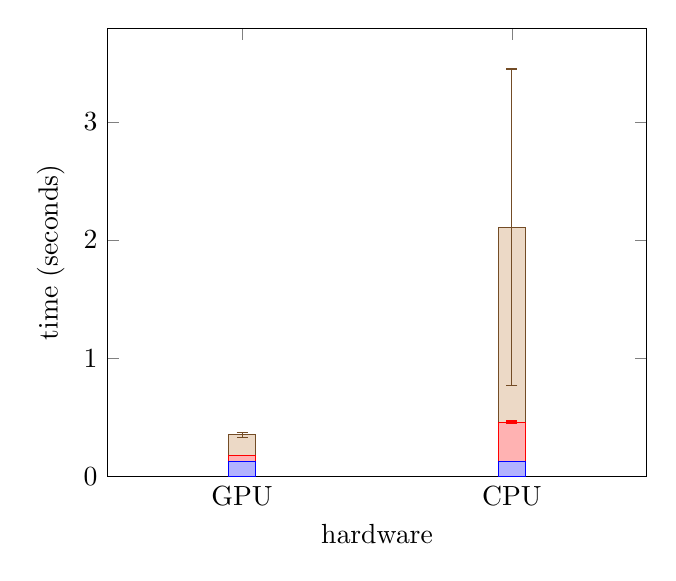
\begin{tikzpicture}
        \begin{axis}[
            ybar stacked,
            xlabel=hardware,
            ylabel=time (seconds),
            ymin=0,
            scaled ticks=false,
            stackedbar/.style = {
                ybar,
                error bars/.cd,
                y dir=both,
                y explicit relative
            },
            xtick={0,1},
            xticklabels={GPU,CPU},
            % nodes near coords,
            x tick label style={align=center},
            enlarge x limits={abs=.5}
        ]
            \addplot+ [stackedbar] coordinates {
                (0,0.12935891456299406) +- (0,0.006906560327033408)
                (1,0.1293111182940452) +- (0,0.006857118137668863)
            };
            \addplot+ [stackedbar] coordinates {
                (0,0.05043862565584919) +- (0,0.0015867081771973946)
                (1,0.33029624063499774) +- (0,0.02197892296588199)
            };
            \addplot+ [stackedbar] coordinates {
                (0,0.17394946628414532) +- (0,0.059306725364273005)
                (1,1.647101882151451) +- (0,0.6361857413955617)
            };
        \end{axis}
    \end{tikzpicture}
\end{figure}

eval on test set
time per inference
\section{Critical appraisal}

% \ifSubfilesClassLoaded{%
% \printglossary[type=\acronymtype]%
% \printbibliography%
% }{}%

\end{document}